\chapter{Mathematische Grundlagen der Kryptographie}
\section{Modulo}
$a$ ganzzahlig durch $m$ dividieren $\rightarrow$ ganzzahligen Quotienten $q$ und den Rest $r$: \\
$a = q \cdot m + r$ \\
$a$ ... Ganzzahl \\
$m$ ... Modul

Für den Rest dieser Gangzahldivision:
$r = a mod m$ (''$a$ modulo $m$)

Beachte:
\begin{itemize}
	\item Es gibt nur $m$ verschiedene Reste bei ganzzahliger Division durch $m$
	\item der Rest $r$ ist nicht negativ! Das gilt auch bei $a$ $<$ 0
\end{itemize}

13 mod 3 = 1 \qquad 13 = 4 $\cdot$ 3 + 1\\
42 mod 5 = 2 \qquad 42 = 8 $\cdot$ 5 + 2\\
42 mod 9 = 6 \qquad 42 = 4 $\cdot$ 9 + 6\\
-13 mod 3 = 2 \qquad -13 = -5 $\cdot$ 3 + 2\\
-42 mod 9 = 3 \qquad -42 = -5 $\cdot$ 9 + 3\\
-36 mod 9 = 0 \qquad -36 = -4 $\cdot$ 9 + 0 \\

mod ist eine \textbf{Rechenoperation}. Sie erhält zwei Argumente, $a$ und $m$, und liefert eine Zahl $r$ als Ergebnis.

\section{Kongruenz modulo $m$}
Wenn 2 ganze Zaheln ($a$, $b$) nach Division durch $m$ den gleichen Rest haben, nennt man sie \textbf{kongruent modulo} $m$ und schreibt:\\
$a \equiv b$ $(mod$ $m)$ \\
Beispiel: $72 \equiv 12$ $(mod$ $10)$ \\
Andere Modulo $m$ sodass $72 \equiv 12$ $(mod$ $m)$: \\
2, 3, 4, 5, 6, 10, 12, 15, 30, 60 \\
Wir sehen, dass man $a$ und $b$ in gewissem Sinne als gleich ansehen kann. Deshalb verwendet man ein Symbol, das an Gleichheit erinnert. Bei der Kongruenz modulo $m$ handelt es sich nicht um eine Rechenoperation sondern um eine \textbf{Aussage}, dass sich nämlich $a$ und $b$ nur um ein Vielfaches des Moduls $m$ unterscheiden: \\
$a \equiv b$ $(mod$ $m)$ $\Leftrightarrow$ $a - b = k \cdot m$

Welche der folgenden Ausdrücke sind wahr?
25 $\equiv$ 0 (mod 5) = $\checkmark$ \\
25 $\equiv$ 20 (mod 5) = $\checkmark$ \\
25 $\equiv$ 20 (mod 10) = \Lightning \\
25 mod 5 = kein Sinn \\

Berechne, falls möglich
25 $\equiv$ 10 = \Lightning \\
25 mod 10 = 5 
\section{Uhrenarithmetik}
Um die Rechenregeln im Zusammenhang mid modulo kennenzulernen, rechnen wir mit Uhrzeiten (modulo 24).
\begin{itemize}
	\item Ein Fertigungsprozess startet um 17 Uhr und dauert 21h. Um welche Uhrzeit endet er? \\
	17 + 21 = 38 $\equiv$ 14 (mod 24) $\rightarrow$ er endet um 14 Uhr
	\item Ein Fertigungsprozess startet um Mitternacht und dauert 38h für den ersten Arbeitsschritt und dann noch einmal 40h für den zweiten. \\
	34 + 40 = 78 $\equiv$ 6 (mod 24) \\
	Alternativ: \\
	38 + 40 $\equiv$ 14 + 40 (mod 24) \\
	38 + 40 $\equiv$ 14 + 16 (mod 24) \\
	38 + 40 $\equiv$ 30 (mod 24) \\
	38 + 40 $\equiv$ 6 (mod 24) \\
	Wir erkennen: \textbf{Bei der Addition modulo $m$ ist es egal, ob vor dem Addieren oder in Zwischenschritten um $m$ reduziert wird}
	\item Ein Arbeitsschritt dauert 22h und muss mit Start um Mitternacht 7-mal durchgeführt werden. Um wie viel Uhr ist er zu Ende? \\
	22 $\cdot$ 7 = 154 $\equiv$ 10 (mod 24) \\
	Alternativ: \\
	22 $\cdot$ 7 $\equiv$ (-2) $\cdot$ (mod 24) $\equiv$ -14 (mod 24) $\equiv$ 10 (mod 24) \\
	Wir erkennen: \textbf{Bei der Multiplikation modulo $m$ ist es egal, ob vor dem Multiplizieren oder in Zwischenschritten um $m$ reduziert wird.}
	\item Daraus folgt, dass \textbf{auch beim Potenzieren die Basis im Voraus um $m$ reduziert werden darf.} \\
	$3^5$ mod 2 = $1^5$ mod 2 = 1 mod 2 = 1
\end{itemize}
	
	(12 + 20) mod 3 = (0 + 2) mod 3 = 2 \\
	(81 - 40) mod 7 = (4 - 5) mod 7 = -1 mod 7 = 6 \\
	(23 $\cdot$ 15) mod 4 = (3 $\cdot$ 3) mod 4 = 9 mod 4 = 1 \\
	(15 $\cdot$ 16 $\cdot$ 17) mod 5 = (0 $\cdot$ 1 $\cdot$ 2) mod 5 = 0 \\
	(18 + 34 $\cdot$ 23) mod 8 = (2 + 2 $\cdot$ 7) mod 8 = (2 + 14) mod 8 = 16 mod 8 = 0 \\
	$17^8$ mod 7 = $3^8$ mod 7 = 6561 mod 7 = 2 
	
	$j^{2}$ = -1 \\
	$j^{3}$ = -j \\
	$j^{4}$ = 1 \\
	$j^{10}$ = -1 \\
	$j^{2024}$ = 1 \\
	$j^{9876543210}$ = -1
	
	(100 + 823) mod 5 = (0 + 3) mod 5 ) 3 \\
	(12 + 5 $\cdot$ 18) mod 7 = (5 + 5 $\cdot$ 4) mod 7 = (5 + 20) mod 7 = (5 + 6) mod 7 = 11 mod 7 = 4 \\
	(23 $\cdot$ 18) mod 5 = (3 $\cdot$ 3) mod 5 = 9 mod 5 = 4 \\
	(19 $\cdot$ 37 $\cdot$ 22) mod 7 = (5 $\cdot$ 2 $\cdot$ 1) mod 7 = 10 mod 7 = 3 \\
	(41 $\cdot$ 23 $\cdot$ 25) mod 9 = (5 $\cdot$ 5 $\cdot$ 7) mod 9 = (25 $\cdot$ 7) mod 9 = (7 $\cdot$ 7) mod 9 = 49 mod 9 = 4 \\
	... \\
	$14^3$ mod 13 = $1^3$ mod 13 = 1 \\
	(212 $\cdot$ $31^2$) mod 21 = (2 $\cdot$ $10^2$) mod 21 = 200 mod 21 = 4 $\cdot$ 50 mod 21 = 4 $\cdot$ 8 mod 21 = 32 mod 21 = 11 \\
	($19^4$ + 14 $\cdot$ $25^5$) mod 8 = ($3^4$ + 6 $\cdot$ $1^5$) mod 8 = 87 mod 8 = 7
\section{Restklassenring $\mathbb{Z}_m$}
......

\subsection{Allgemeine Eigenschaften der Restklassenringe, algebraische Strukturen}
......

\section{Berechnung des ggT}
Die berechnung des \textbf{größten gemeinsamen Teiler} kann durch unterschiedliche Möglichkeiten berechnet werden. Durchgeführt mit $a$ = 2079 und $b$ = 735.

\subsection{Primfaktorzerlegung beider Zahlen}
Sehr aufwändig! Man zerlegt beide Zahlen in ihre Primfaktoren. Der ggT wird aus allen gemeinsamen Primfaktoren gebildet (Taucht ein Primfaktor mehrfach auf, wird er so oft verwendet, wie er in beiden Zahlen vorkommt): \\
2079 = 3 $\cdot$ 693 = 3 $\cdot$ 3 $\cdot$ 231 = 3 $\cdot$ 3 $\cdot$ 3 $\cdot$ 7 $\cdot$ 11 \\
735 = 3 $\cdot$ 245 = 5 $\cdot$ 3 $\cdot$ 49 = 7 $\cdot$ 7 $\cdot$ 5 $\cdot$ 3 \\
ggT(2079, 735) = 3 $\cdot$ 7 = 21

\subsection{Euklidischer Algorithmus}
Man subtrahiert immer die kleinere von der größteren Zahl und fährt mit kleinerer Zahl und Differenz fort. Die letzte Zahl, die nicht durch subtrahieren auf 0 führt, ist der ggT.
\begin{tabular}{rllll}
	2079 - 735 & = 1344 &  & 2079 mod 735 & = 609 \\
	1344 - 735 & = 609 &  & 735 mod 609 & = 126 \\
	735 - 609 & = 126 &  & 609 mod 126 & = 105 \\
	609 - 126 & = 483 &  & 126 mod 105 & = 21 \\
	483 - 126 & = 357 &  & (105 mod 21 & = 0) \\
	357 - 126 & = 231 &  &  &  \\
	231 - 126 & = 105 &  &  &  \\
	126 - 105 & = 21 &  &  &  \\
	105 - 21 & = 84 &  &  &  \\
	84 - 21 & = 63 &  &  &  \\
	63 - 21 & = 42 &  &  &  \\
	42 - 21 & = 21 &  &  &  \\
	(21 - 21 & = 0) &  &  &  \\
\end{tabular}

$\rightarrow$ ggT(1079, 735) = 21 \\
Entweder durch Subtrahieren oder Modulo rechnen.

\subsection{Erweiterter euklidischer Algorithmus}
Mit dem erweiterten euklidischer Algorithmus kann das Invers einer Zahl berechnet werden. Hier wird das ggT als Vielfachsumme von $a$ und $b$ angeschrieben: \\
$ggT$($a$, $b$) = $s$ $\cdot$ $a$ + $t$ $\cdot$ $b$

Links wird der normale euklidische Algorithmus durchgeführt. Jedoch notieren wir, wie oft die kleinere Zahl in die größere passt. Diese Zahl (mal -1) multiplizieren wird mit der aktuellen Reihe und addieren die Multiplizierte Reihe mit der oberen.

\begin{tabular}{rcccl}
	2079 = & 1 $\cdot$ 2079 & + & 0 $\cdot$ 735 &  \\
	735 = & 0 $\cdot$ 2079 & + & 1 $\cdot$ 735 & $|$ $\cdot$ -2 \\
	609 = & 1 $\cdot$ 2079 & + & -2 $\cdot$ 735 & $|$ $\cdot$ -1 \\
	126 = & -1 $\cdot$ 2079 & + & 3 $\cdot$ 735 & $|$ $\cdot$ -4 \\
	105 = & 5 $\cdot$ 2079 & + & -14 $\cdot$ 735 & $|$ $\cdot$ -1 \\
	21 = & -6 $\cdot$ 2079 & + & 14 $\cdot$ 735 & \\
	0 = &  & &  & \\
\end{tabular}

$\rightarrow$ ggT(1079, 735) = 21 \\

Ein Beispiel zur Ermittlung eines Invers: Inverse von $\overline{\text{5}}$ in $\mathbb{Z}_{26}$ \\
\begin{tabular}{rcccl}
	26 = & 1 $\cdot$ 26 & + & 0 $\cdot$ 5 &  \\
	5 = & 0 $\cdot$ 26 & + & 1 $\cdot$ 5 & $|$ $\cdot$ -5 \\
	1 = & 1 $\cdot$ 26 & + & -5 $\cdot$ 5 & $|$ fertig, da 1 links herauskommt
\end{tabular} \\
... daraus 
\begin{itemize}
	\item ggT(26, 5) = 1, daher ist $\overline{\text{5}}$ in $\mathbb{Z}_{26}$ invertierbar
	\item[] ... würde anstatt 1 in der letzten Zeil 0 herauskommen, gäbe es kein Invers zu dieser Zahl
	\item das Inverse von $\overline{\text{5}}$ ist $\overline{\text{-5}}$ $\rightarrow$ -5 + 26 = \textbf{21}
\end{itemize}

\section{Eulersche Phi-Funktion}
Die Phi-Funktion $\varphi$($n$) gibt die Anzahl der invertierbaren Elemente von $\mathbb{Z}_{n}$.

\begin{itemize}
	\item Ist $n$ prim, gilt $\varphi$($n$) = $n$ - 1
	\item Ist $n$ nicht prim $\rightarrow$ Primfaktorzerlegung, $\varphi$ mit jeder Primzahl durchführen; bei mehrfachen vorkommen von Primzahlen nur einmal $\varphi$ verwenden, anschließend alle multiplizieren. Beispiel \\
	 $\varphi$(810) = $\varphi$(2$\cdot$3$\cdot$3$\cdot$3$\cdot$3$\cdot$5) = $\varphi$(2) $\cdot$ $\varphi$(3 $\cdot$ 3 $\cdot$ 3 $\cdot$ 3) $\cdot$ $\varphi$(5) = 1 $\cdot$ 2 $\cdot$ 3 $\cdot$ 3 $\cdot$ 3 $\cdot$ 4 = 216 \\
	 ... 216 Zahlen sind in $\mathbb{Z}_{810}$ teilerfremd und 216 invertierbare Elemente.
\end{itemize}

\textbf{Das Berechnen von Invers ist leicht. Das Bestimmen von wie viele invertierbare Elemente es gibt ist bei Primzahlen einfach, sonst aber (bei großen Zahlen besonders) schwer, da man die Primfaktorzerlegung durchführen muss.}

\section{Einweg- und Falltürfunktionen}
Eine Funktion weist zu jeder \textit{Definitionsmenge} eine \textit{Wertemenge}. Für die Verschlüsselung ist dies jedoch ungünstig, da man von der verschlüsselten Nachricht einfach auf dem Klartext kommen würde.
\begin{figure}[H]
	\centering
	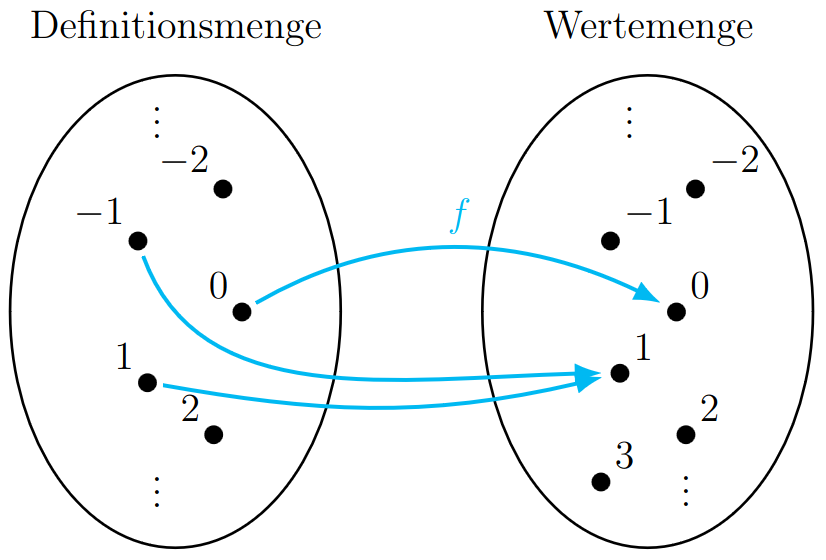
\includegraphics[width=0.8\linewidth]{figures/normal_func.png}
	\caption{Definitionsmenge und Wertemenge einer normalen Funktion}
\end{figure}

Eine \textbf{umkehrbare Funktion} verwendet jede Wertemenge einmal. Daher ist das Umkehren aufgrund der Eindeutigkeit auch wieder einfach und für die Verschlüsselung ungünstig.
\begin{figure}[H]
	\centering
	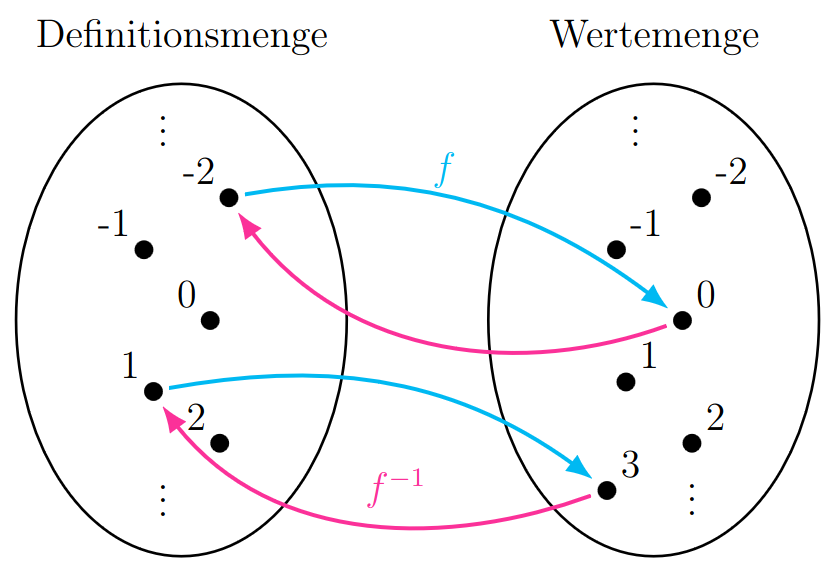
\includegraphics[width=0.8\linewidth]{figures/umkehr_func.png}
	\caption{Definitionsmenge und Wertemenge einer umkehrbaren Funktion}
\end{figure}

Eine \textbf{Einwegfunktion} ist zwar theoretisch umkehrbar, dies ist aber sehf aufwändig.
\begin{figure}[H]
	\centering
	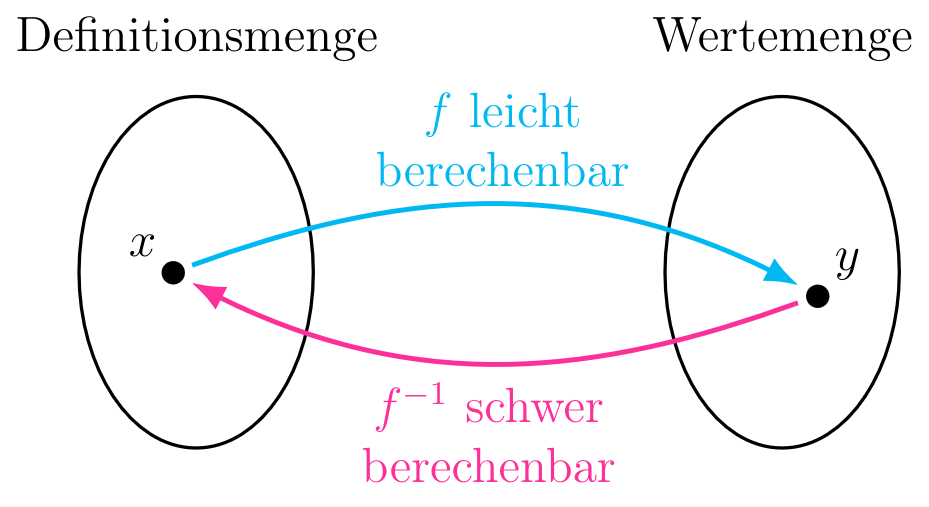
\includegraphics[width=0.8\linewidth]{figures/einweg_func.png}
	\caption{Definitionsmenge und Wertemenge einer Einwegfunktion}
\end{figure}
Zur Verschlüsselung kann eine Einwegfunktion jedoch auch nicht verwendet werden, da die Umkehrung sehr lange dauern würde (Beispiel Kommunikation zwischen \textit{Alice} und \textit{Bob}).

Eine \textbf{Falltürfunktion} ist allgemein sehr aufwändig zum umkehren, aber sehr einfach mit Zusatzinformation.
\begin{figure}[H]
	\centering
	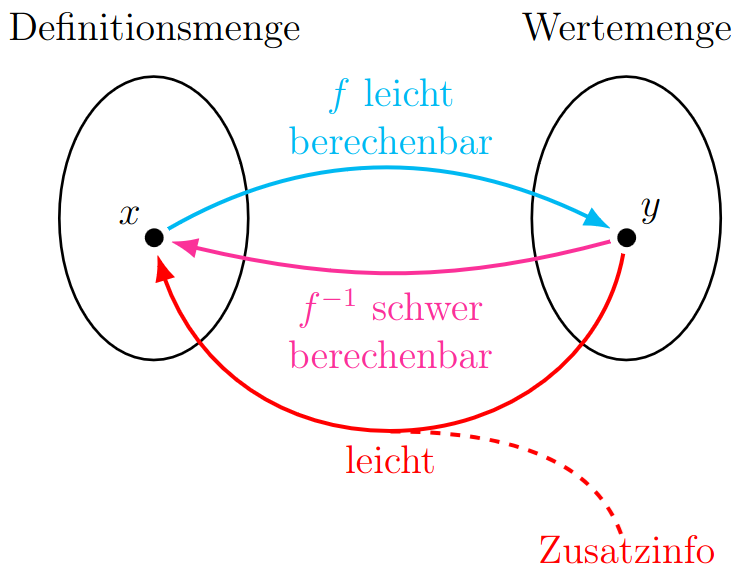
\includegraphics[width=0.8\linewidth]{figures/falltur_func.png}
	\caption{Definitionsmenge und Wertemenge einer Falltürfunktion}
\end{figure}

\section{Modulares Potenzieren und diskreter Logarithmus}
\subsection{Modulares Potenzieren}
......

\subsection{Diskreter Logarithmus}
......

\subsection{Aufwand des modularen Potenzieren}
......

\subsection{Aufwand der Berechnung des diskreten Logarithmus}
......

